\section{eo\-Pop$<$ EOT $>$ Class Template Reference}
\label{classeo_pop}\index{eoPop@{eoPop}}
A std::vector of {\bf EO}{\rm (p.\,\pageref{class_e_o})} object, to be used in all algorithms (selectors, operators, replacements, ...).  


{\tt \#include $<$eo\-Pop.h$>$}

Inheritance diagram for eo\-Pop$<$ EOT $>$::\begin{figure}[H]
\begin{center}
\leavevmode
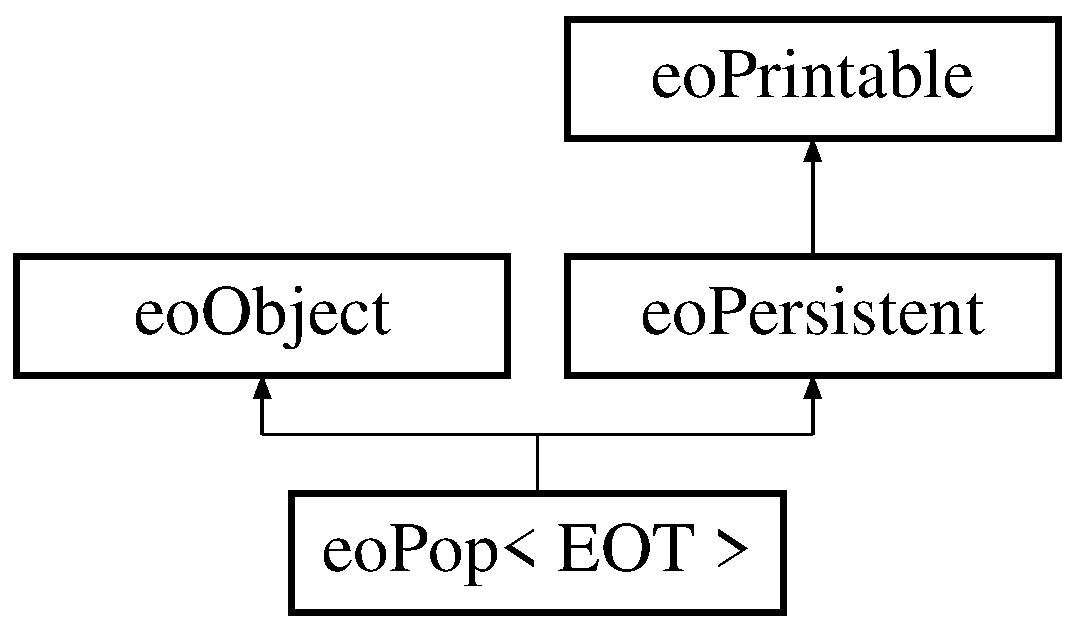
\includegraphics[height=3cm]{classeo_pop}
\end{center}
\end{figure}
\subsection*{Public Types}
\begin{CompactItemize}
\item 
typedef EOT::Fitness {\bf Fitness}\label{classeo_pop_w0}

\item 
typedef EOT::fitness\_\-traits {\bf fitness\_\-traits}\label{classeo_pop_w1}

\end{CompactItemize}
\subsection*{Public Member Functions}
\begin{CompactItemize}
\item 
{\bf eo\-Pop} ()
\begin{CompactList}\small\item\em Default ctor. \item\end{CompactList}\item 
{\bf eo\-Pop} (unsigned \_\-pop\-Size, {\bf eo\-Init}$<$ {\bf EOT} $>$ \&\_\-chrom\-Init)
\begin{CompactList}\small\item\em Ctor for the initialization of chromosomes. \item\end{CompactList}\item 
void {\bf append} (unsigned \_\-new\-Pop\-Size, {\bf eo\-Init}$<$ {\bf EOT} $>$ \&\_\-chrom\-Init)
\begin{CompactList}\small\item\em appstd::ends random guys at end of pop. \item\end{CompactList}\item 
{\bf eo\-Pop} (std::istream \&\_\-is)
\begin{CompactList}\small\item\em Ctor from an std::istream; reads the population from a stream, each element should be in different lines. \item\end{CompactList}\item 
virtual {\bf $\sim$eo\-Pop} ()\label{classeo_pop_a4}

\begin{CompactList}\small\item\em Empty Dtor. \item\end{CompactList}\item 
void {\bf sort} (void)
\begin{CompactList}\small\item\em sort the population. \item\end{CompactList}\item 
void {\bf sort} (std::vector$<$ const {\bf EOT} $\ast$ $>$ \&result) const \label{classeo_pop_a6}

\begin{CompactList}\small\item\em creates a std::vector$<$EOT$\ast$$>$ pointing to the individuals in descending order \item\end{CompactList}\item 
void {\bf shuffle} (void)
\begin{CompactList}\small\item\em shuffle the population. \item\end{CompactList}\item 
void {\bf shuffle} (std::vector$<$ const {\bf EOT} $\ast$ $>$ \&result) const \label{classeo_pop_a8}

\begin{CompactList}\small\item\em creates a std::vector$<$EOT$\ast$$>$ pointing to the individuals in random order \item\end{CompactList}\item 
{\bf eo\-Pop}$<$ {\bf EOT} $>$::iterator {\bf it\_\-best\_\-element} ()\label{classeo_pop_a9}

\begin{CompactList}\small\item\em returns an iterator to the best individual DOES NOT MOVE ANYBODY \item\end{CompactList}\item 
const {\bf EOT} \& {\bf best\_\-element} () const \label{classeo_pop_a10}

\begin{CompactList}\small\item\em returns an iterator to the best individual DOES NOT MOVE ANYBODY \item\end{CompactList}\item 
const {\bf EOT} \& {\bf worse\_\-element} () const \label{classeo_pop_a11}

\begin{CompactList}\small\item\em returns a const reference to the worse individual DOES NOT MOVE ANYBODY \item\end{CompactList}\item 
{\bf eo\-Pop}$<$ {\bf EOT} $>$::iterator {\bf it\_\-worse\_\-element} ()\label{classeo_pop_a12}

\begin{CompactList}\small\item\em returns an iterator to the worse individual DOES NOT MOVE ANYBODY \item\end{CompactList}\item 
{\bf eo\-Pop}$<$ {\bf EOT} $>$::iterator {\bf nth\_\-element} (int nth)
\begin{CompactList}\small\item\em slightly faster algorithm than sort to find all individuals that are better than the nth individual. \item\end{CompactList}\item 
Fitness {\bf nth\_\-element\_\-fitness} (int which) const \label{classeo_pop_a14}

\begin{CompactList}\small\item\em returns the fitness of the nth element \item\end{CompactList}\item 
void {\bf nth\_\-element} (int which, std::vector$<$ const {\bf EOT} $\ast$ $>$ \&result) const \label{classeo_pop_a15}

\begin{CompactList}\small\item\em const nth\_\-element function, returns pointers to sorted individuals up the the nth \item\end{CompactList}\item 
void {\bf swap} ({\bf eo\-Pop}$<$ {\bf EOT} $>$ \&other)\label{classeo_pop_a16}

\begin{CompactList}\small\item\em does STL swap with other pop \item\end{CompactList}\item 
virtual void {\bf sorted\-Print\-On} (std::ostream \&\_\-os) const 
\begin{CompactList}\small\item\em Prints sorted pop but does NOT modify it! \item\end{CompactList}\item 
virtual void {\bf print\-On} (std::ostream \&\_\-os) const 
\begin{CompactList}\small\item\em Write object. \item\end{CompactList}\item 
virtual void {\bf invalidate} ()\label{classeo_pop_a19}

\item 
void {\bf sort} ()\label{classeo_pop_a21}

\item 
void {\bf scale} ()\label{classeo_pop_a22}

\item 
void {\bf set\-Perf2Worth} ({\bf eo\-Perf2Worth}$<$ {\bf EOT} $>$ \&\_\-p2w)\label{classeo_pop_a23}

\item 
void {\bf set\-Perf2Worth} ({\bf eo\-Perf2Worth}$<$ {\bf EOT} $>$ $\ast$\_\-p2w)\label{classeo_pop_a24}

\item 
{\bf eo\-Perf2Worth}$<$ {\bf EOT} $>$ $\ast$ {\bf get\-Perf2Worth} ()\label{classeo_pop_a25}

\item 
void {\bf swap} ({\bf eo\-Pop}$<$ {\bf EOT} $>$ \&other)\label{classeo_pop_a26}

\end{CompactItemize}
\begin{Indent}{\bf Methods from eo\-Object}\par
\begin{CompactItemize}
\item 
virtual void {\bf read\-From} (std::istream \&\_\-is)
\begin{CompactList}\small\item\em Read object. \item\end{CompactList}\item 
virtual std::string {\bf class\-Name} () const 
\begin{CompactList}\small\item\em Inherited from {\bf eo\-Object}{\rm (p.\,\pageref{classeo_object})}. \item\end{CompactList}\end{CompactItemize}
\end{Indent}
\subsection*{Private Attributes}
\begin{CompactItemize}
\item 
{\bf eo\-Perf2Worth}$<$ {\bf EOT} $>$ $\ast$ {\bf p2w}\label{classeo_pop_r0}

\end{CompactItemize}


\subsection{Detailed Description}
\subsubsection*{template$<$class EOT$>$ class eo\-Pop$<$ EOT $>$}

A std::vector of {\bf EO}{\rm (p.\,\pageref{class_e_o})} object, to be used in all algorithms (selectors, operators, replacements, ...). 

We have no idea if a population can be some other thing that a std::vector, but if somebody thinks of it, this concrete implementation can be moved to \char`\"{}generic\char`\"{} and an abstract Population interface be provided.

The template can be instantiated with anything that accepts a \char`\"{}size\char`\"{} and {\bf eo\-Init}{\rm (p.\,\pageref{classeo_init})} derived object. in the ctor. EOT must also have a copy ctor, since temporaries are created and then passed to the {\bf eo\-Init}{\rm (p.\,\pageref{classeo_init})} object 



Definition at line 54 of file eo\-Pop.h.

\subsection{Constructor \& Destructor Documentation}
\index{eoPop@{eo\-Pop}!eoPop@{eoPop}}
\index{eoPop@{eoPop}!eoPop@{eo\-Pop}}
\subsubsection{\setlength{\rightskip}{0pt plus 5cm}template$<$class EOT$>$ {\bf eo\-Pop}$<$ {\bf EOT} $>$::{\bf eo\-Pop} ()\hspace{0.3cm}{\tt  [inline]}}\label{classeo_pop_a0}


Default ctor. 

Creates empty pop

Definition at line 68 of file eo\-Pop.h.\index{eoPop@{eo\-Pop}!eoPop@{eoPop}}
\index{eoPop@{eoPop}!eoPop@{eo\-Pop}}
\subsubsection{\setlength{\rightskip}{0pt plus 5cm}template$<$class EOT$>$ {\bf eo\-Pop}$<$ {\bf EOT} $>$::{\bf eo\-Pop} (unsigned {\em \_\-pop\-Size}, {\bf eo\-Init}$<$ {\bf EOT} $>$ \& {\em \_\-chrom\-Init})\hspace{0.3cm}{\tt  [inline]}}\label{classeo_pop_a1}


Ctor for the initialization of chromosomes. 

\begin{Desc}
\item[Parameters:]
\begin{description}
\item[{\em \_\-pop\-Size}]total population size \item[{\em \_\-chrom\-Init}]Initialization routine, produces EO's, needs to be an {\bf eo\-Init}{\rm (p.\,\pageref{classeo_init})}\end{description}
\end{Desc}


Definition at line 75 of file eo\-Pop.h.\index{eoPop@{eo\-Pop}!eoPop@{eoPop}}
\index{eoPop@{eoPop}!eoPop@{eo\-Pop}}
\subsubsection{\setlength{\rightskip}{0pt plus 5cm}template$<$class EOT$>$ {\bf eo\-Pop}$<$ {\bf EOT} $>$::{\bf eo\-Pop} (std::istream \& {\em \_\-is})\hspace{0.3cm}{\tt  [inline]}}\label{classeo_pop_a3}


Ctor from an std::istream; reads the population from a stream, each element should be in different lines. 

\begin{Desc}
\item[Parameters:]
\begin{description}
\item[{\em \_\-is}]the stream \end{description}
\end{Desc}


Definition at line 113 of file eo\-Pop.h.

\subsection{Member Function Documentation}
\index{eoPop@{eo\-Pop}!append@{append}}
\index{append@{append}!eoPop@{eo\-Pop}}
\subsubsection{\setlength{\rightskip}{0pt plus 5cm}template$<$class EOT$>$ void {\bf eo\-Pop}$<$ {\bf EOT} $>$::append (unsigned {\em \_\-new\-Pop\-Size}, {\bf eo\-Init}$<$ {\bf EOT} $>$ \& {\em \_\-chrom\-Init})\hspace{0.3cm}{\tt  [inline]}}\label{classeo_pop_a2}


appstd::ends random guys at end of pop. 

Can be used to initialize it pop is empty

\begin{Desc}
\item[Parameters:]
\begin{description}
\item[{\em \_\-pop\-Size}]total population size \item[{\em \_\-chrom\-Init}]Initialization routine, produces EO's, needs to be an {\bf eo\-Init}{\rm (p.\,\pageref{classeo_init})}\end{description}
\end{Desc}


Definition at line 91 of file eo\-Pop.h.

Referenced by eo\-Easy\-EA$<$ EOT $>$::operator()().\index{eoPop@{eo\-Pop}!sort@{sort}}
\index{sort@{sort}!eoPop@{eo\-Pop}}
\subsubsection{\setlength{\rightskip}{0pt plus 5cm}template$<$class EOT$>$ void {\bf eo\-Pop}$<$ {\bf EOT} $>$::sort (void)\hspace{0.3cm}{\tt  [inline]}}\label{classeo_pop_a5}


sort the population. 

Use this member to sort in order of descending Fitness, so the first individual is the best! 

Definition at line 133 of file eo\-Pop.h.

Referenced by eo\-Truncated\-Select\-Many$<$ EOT $>$::operator()(), eo\-Reduce\-Merge\-Reduce$<$ EOT $>$::operator()(), eo\-Ranking$<$ EOT $>$::operator()(), eo\-PBILAdditive$<$ EOT $>$::operator()(), eo\-Check\-Point$<$ EOT $>$::operator()(), eo\-Sequential\-Select$<$ EOT $>$::setup(), and eo\-Pop$<$ Dummy $>$::sorted\-Print\-On().\index{eoPop@{eo\-Pop}!shuffle@{shuffle}}
\index{shuffle@{shuffle}!eoPop@{eo\-Pop}}
\subsubsection{\setlength{\rightskip}{0pt plus 5cm}template$<$class EOT$>$ void {\bf eo\-Pop}$<$ {\bf EOT} $>$::shuffle (void)\hspace{0.3cm}{\tt  [inline]}}\label{classeo_pop_a7}


shuffle the population. 

Use this member to put the population in random order 

Definition at line 152 of file eo\-Pop.h.

Referenced by eo\-Truncated\-Select\-Many$<$ EOT $>$::operator()(), eo\-Random\-Split$<$ EOT $>$::operator()(), eo\-Random\-Reduce$<$ EOT $>$::operator()(), eo\-Elite\-Sequential\-Select$<$ EOT $>$::setup(), and eo\-Sequential\-Select$<$ EOT $>$::setup().\index{eoPop@{eo\-Pop}!nth_element@{nth\_\-element}}
\index{nth_element@{nth\_\-element}!eoPop@{eo\-Pop}}
\subsubsection{\setlength{\rightskip}{0pt plus 5cm}template$<$class EOT$>$ {\bf eo\-Pop}$<${\bf EOT}$>$::iterator {\bf eo\-Pop}$<$ {\bf EOT} $>$::nth\_\-element (int {\em nth})\hspace{0.3cm}{\tt  [inline]}}\label{classeo_pop_a13}


slightly faster algorithm than sort to find all individuals that are better than the nth individual. 

INDIVIDUALS ARE MOVED AROUND in the pop. 

Definition at line 201 of file eo\-Pop.h.

Referenced by eo\-Deterministic\-Survive\-And\-Die$<$ EOT $>$::operator()(), eo\-Truncate\-Split$<$ EOT $>$::operator()(), eo\-Reduce\-Merge\-Reduce$<$ EOT $>$::operator()(), eo\-Truncate$<$ EOT $>$::operator()(), eo\-Elitism$<$ EOT $>$::operator()(), and eo\-Truncated\-Select\-One$<$ EOT $>$::setup().\index{eoPop@{eo\-Pop}!sortedPrintOn@{sortedPrintOn}}
\index{sortedPrintOn@{sortedPrintOn}!eoPop@{eo\-Pop}}
\subsubsection{\setlength{\rightskip}{0pt plus 5cm}template$<$class EOT$>$ virtual void {\bf eo\-Pop}$<$ {\bf EOT} $>$::sorted\-Print\-On (std::ostream \& {\em \_\-os}) const\hspace{0.3cm}{\tt  [inline, virtual]}}\label{classeo_pop_a17}


Prints sorted pop but does NOT modify it! 

\begin{Desc}
\item[Parameters:]
\begin{description}
\item[{\em \_\-os}]A std::ostream. \end{description}
\end{Desc}


Definition at line 247 of file eo\-Pop.h.\index{eoPop@{eo\-Pop}!printOn@{printOn}}
\index{printOn@{printOn}!eoPop@{eo\-Pop}}
\subsubsection{\setlength{\rightskip}{0pt plus 5cm}template$<$class EOT$>$ virtual void {\bf eo\-Pop}$<$ {\bf EOT} $>$::print\-On (std::ostream \& {\em \_\-os}) const\hspace{0.3cm}{\tt  [inline, virtual]}}\label{classeo_pop_a18}


Write object. 

It's called print\-On since it prints the object \_\-on\_\- a stream. \begin{Desc}
\item[Parameters:]
\begin{description}
\item[{\em \_\-os}]A std::ostream. \end{description}
\end{Desc}


Implements {\bf eo\-Printable} {\rm (p.\,\pageref{classeo_printable_a1})}.

Definition at line 262 of file eo\-Pop.h.\index{eoPop@{eo\-Pop}!readFrom@{readFrom}}
\index{readFrom@{readFrom}!eoPop@{eo\-Pop}}
\subsubsection{\setlength{\rightskip}{0pt plus 5cm}template$<$class EOT$>$ virtual void {\bf eo\-Pop}$<$ {\bf EOT} $>$::read\-From (std::istream \& {\em \_\-is})\hspace{0.3cm}{\tt  [inline, virtual]}}\label{classeo_pop_z19_0}


Read object. 

The EOT class must have a ctor from a stream; \begin{Desc}
\item[Parameters:]
\begin{description}
\item[{\em \_\-is}]A std::istream. \end{description}
\end{Desc}


Implements {\bf eo\-Persistent} {\rm (p.\,\pageref{classeo_persistent_a1})}.

Definition at line 274 of file eo\-Pop.h.

Referenced by eo\-Pop$<$ Dummy $>$::eo\-Pop().\index{eoPop@{eo\-Pop}!className@{className}}
\index{className@{className}!eoPop@{eo\-Pop}}
\subsubsection{\setlength{\rightskip}{0pt plus 5cm}template$<$class EOT$>$ virtual std::string {\bf eo\-Pop}$<$ {\bf EOT} $>$::class\-Name (void) const\hspace{0.3cm}{\tt  [inline, virtual]}}\label{classeo_pop_z19_1}


Inherited from {\bf eo\-Object}{\rm (p.\,\pageref{classeo_object})}. 

Returns the class name. \begin{Desc}
\item[See also:]{\bf eo\-Object}{\rm (p.\,\pageref{classeo_object})} \end{Desc}


Implements {\bf eo\-Object} {\rm (p.\,\pageref{classeo_object_a1})}.

Definition at line 289 of file eo\-Pop.h.

Referenced by eo\-Check\-Point$<$ EOT $>$::all\-Class\-Names().

The documentation for this class was generated from the following files:\begin{CompactItemize}
\item 
eo\-Pop.h\item 
fitness\_\-traits.cpp\end{CompactItemize}
